\documentclass[10pt, oneside, letterpaper]{article}
\usepackage[utf8]{inputenc}

\usepackage{authblk}
	\setcounter{Maxaffil}{0}
	\renewcommand\Affilfont{\itshape\small}
\usepackage{float}
\usepackage[margin=1.3in]{geometry}
\usepackage{graphicx}
	\graphicspath{ {img/} }
\usepackage[colorlinks=true, linkcolor=blue, citecolor=blue]	{hyperref}
\usepackage{indentfirst}
	\setlength{\parindent}{15pt}
\usepackage{multicol}
\usepackage{ragged2e}
\usepackage[raggedright]{titlesec}
\usepackage{verbatim}

% Second set of package loads
\usepackage{apacite}  % Must occur after hyperref

\title{\textbf{Clean Energy and Sustainable Cities:\\A Synergistic Approach}}
\author{Jeffrey Leung}
\affil{Simon Fraser University}
\date{October 6, 2019}

\begin{document}

	\maketitle

	\begin{abstract}
		This paper is an assignment for SEE 101W: Process, Form and Convention in Professional Genres. This paper compares and contrasts two of the United Nations Sustainable Development Goals; Sustainable Cities, and Affordable and Clean Energy. Their objectives and means are described in addition to their relevances to sustainability. The comparisons reveal interdependencies which can be leveraged to create more effective and impactful policies and implementation of such policies. These interdependencies include transportation and urban clean energy, both of which are demonstrated to have been effectively implemented previously.
	\end{abstract}

	\begin{multicols}{2}

	\section{Introduction}

	Over the past several decades, the worldwide climate crisis has rapidly escalated to clear undeniability. Community grassroots movements and global protests attempt to spur drastic political action as cities and industries pivot towards sustainable initiatives at ever-increasing speeds. In 2015, the United Nations established 17 ambitious objectives to achieve by 2030 for a sustainable free world, termed the Sustainable Development Goals \cite{UN2015}. From these 17 goals, Goal 7: Affordable and Clean Energy and Goal 11: Sustainable Cities have been chosen to be compared, contrasted, and strategized. This paper will discuss definitions of and distinctions between the objectives of affordable clean energy and sustainable cities, as well as provide concrete examples to illustrate the interplay and interdependence of the goals.

	\section{Definitions and Distinctions}
	
	\subsection{Divergences}

	The objectives of achieving affordable and clean energy, and sustainable cities diverge in a number of ways. Establishing affordable and clean energy can be described as "ensuring universal access to affordable, reliable and modern energy services" \cite{UNcities}. Conventional usages of fossil fuels should be replaced with energy sources which do not emit greenhouse gases or are carbon-neutral, and all people should have universal and reasonable access to this energy. In contrast, creating sustainable cities can be described as building a better long-term socioeconomic quality of life for citizens by designing urban environments to be sustainable.  The divergence is clearer when comparing the spheres of influence of each goal. Clean energy focuses on the root energy sources which are either sustainable – for example, wind, hydropower, geothermal, and bioenergy sources \cite{Blakers2015} – or utilizing carbon capture and storage strategies. This energy can be generally applied to industrial or urban use. Comparatively, designing sustainable cities utilizes these clean energy sources for electricity or transportation but inevitably includes differing components such as infrastructure and housing. Finally, the impact of improving our energy methodology is primarily in reducing greenhouse gases, as the emissions from fossil fuels in the energy sector consist of over 60\% of global greenhouse gas emissions \cite{Blakers2015}. However, the impact of building sustainable cities is directly upon the residential and local experiences of citizens. Rather than being globally environmental, the results are a visible and personal motivation compared to the distantly nebulous threat of increasing greenhouse gases.
	
	\begin{figure}[H]
		\centering
		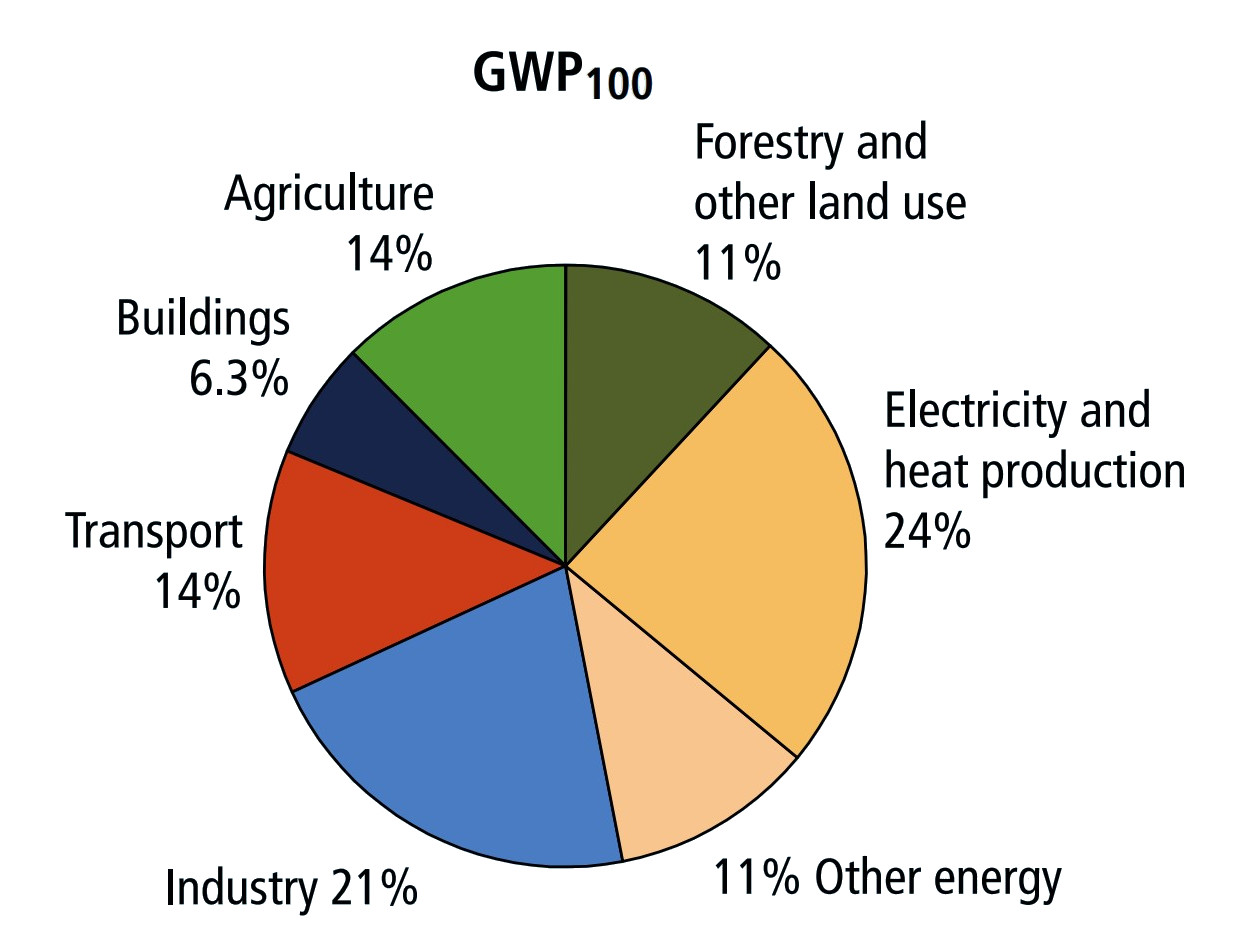
\includegraphics[width=\linewidth]{global-warming-potential}
		\caption{Global Warming Potentials contribution to greenhouse gas emissions in the year 2010. \protect\cite{Pachauri2014}. p. 88.}
		\label{fig:global-warming-potentials}
	\end{figure}
	
	\subsection{Convergences}
	
	The convergence of these two objectives is in how they both involve the use of clean renewable energy for reducing short-term environmental impacts and improving long-term environmental conservation efforts. Affordable and clean energy is among the most significant components to implementing successful sustainable cities. Figure 1 shows how urban consumptions of energy - namely, buildings, transport, and electricity/heat production - consisted of over 44\% of global warming potential in 2010. There are many intersections such as these which could be identified to create effective strategies which affect both the goals of clean energy and sustainable cities.
	
	\section{Interdependence and Synergy}
	
	While similarities and differences have been discussed, in practice these two goals can influence each other significantly in policy and implementation. Generally, these goals are seen to be complementary to each other. For example, a study conducted by \citeA{Mroczek2014} on the social attitudes towards renewable energy sources demonstrated a clear majority of those who support local development of the energy source and wind industry. The reasons included health, environment, labour industry, and energy security. In fact, 20\% of respondents were willing to pay additional electricity costs for renewable energy to obtain its benefits. This demonstrates the correlation of public support of the generation of renewable energy with their sustainable urban benefits. Projects for renewable energy could be promoted effectively through its urban impacts, which would create personal connection and garner stronger public support.
	
	\subsection{A Synergistic Approach: Transportation}
	
	The analysis of various socioeconomic deficiencies also presents a key opportunity to capitalize on the convergence of multiple Sustainable Development Goals, achieving multiple objectives simultaneously. One area where both clean energy and sustainable cities have significant potential to be impacted is public transport. Fossil-fuel based individual transportation is used by many urban commuters; a transition to high-capacity rapid transit systems utilizing hybrid or electric energy creates a meaningful impact on the emission of greenhouse gases created by these commuters. Cities are continuing to explore policies and programs such as the Environmentally Sustainable Transport strategy in Japan to create sufficient public transit, park-and-ride facilities, and walkable community designs \cite{Sakamoto2008}. In addition, Sakamoto describes local workshops which are held to encourage and generate public input for designing community transit systems to best serve the public. These are commendable approaches to using cleaner and less energy while improving sustainable urban development, though they must always be balanced.
	
	\subsection{A Synergistic Approach: 2020 Olympic Games}
	
	An even clearer example for a beneficial independence is illustrated by the 2020 Olympic Games. Tokyo committed to using only renewable energy for its upcoming Olympic Games through minimizing resource usage, purchasing from renewable sources, and installing thousands of road-embedded solar panels \cite{Movellan2015}. The urban motivation to improve quality of life is augmented by the increase of available and affordable sustainable energy in this context. Often, the cost of implementing clean energy is a heavy economic and political burden. Redesigning infrastructure and displacing longstanding fossil fuel industries causes great strain which is why the immediate effects of sustainable urban development are an effective offset to these detriments. Strategies like the aforementioned projects demonstrate an increase in sustainable urbanity and a simultaneous decrease in the reliance on fossil fuel energy.
	
	\begin{figure}[H]
		\centering
		
\includegraphics[width=\linewidth]{tokyo-stadium}
		\caption{Render of the Japan National Stadium. \protect\cite{Virtuoso2018}.}
		\label{fig:tokyo-stadium}
	\end{figure}
	
	\section{Conclusion}
	
	Although the progression of clean energy is directed towards ecological improvement and the creation of sustainable cities is directed towards urban experience development, they converge clearly in the ideal vision of a green and accessible city. An understanding of their intersections and differences is critical to the creation of policies which can provide a net increase in socioeconomic and ecological benefit. The clearest example is how the development of policies for sustainable energy used by cities can offset the political and economical deficits which result from the enactment of said policies. The combination of universal access to clean energy, management of sustainable resource consumption, and reprioritization of public funding towards sustainable urbanization can be an effective and balanced strategy to accelerate urban development and environmental awareness, providing citizens with a robust platform upon which to build a better life.

	\end{multicols}

	\nocite{*}  % Show all citations, referenced or not
	\bibliographystyle{apacite}
	{\RaggedRight
		\bibliography{clean-energy-and-sustainable-cities}
	}

\end{document}
